% !TEX TS-program = pdflatex
% !TEX encoding = UTF-8 Unicode
% !TEX spellcheck = en_US

% This is a simple template for a LaTeX document using the "article" class.
% See "book", "report", "letter" for other types of document.

\documentclass[11pt]{article} % use larger type; default would be 10pt

\usepackage{fancyvrb}
\usepackage{multicol}

\usepackage[utf8]{inputenc} % set input encoding (not needed with XeLaTeX)
\usepackage{amssymb}
%%% Examples of Article customizations
% These packages are optional, depending whether you want the features they provide.
% See the LaTeX Companion or other references for full information.

%%% PAGE DIMENSIONS
\usepackage{geometry} % to change the page dimensions
\geometry{a4paper} % or letterpaper (US) or a5paper or....
% \geometry{margin=2in} % for example, change the margins to 2 inches all round
% \geometry{landscape} % set up the page for landscape
%   read geometry.pdf for detailed page layout information
% \usepackage{amsmath}
\usepackage{graphicx} % support the \includegraphics command and options

% \usepackage[parfill]{parskip} % Activate to begin paragraphs with an empty line rather than an indent

%%% PACKAGES
% \usepackage{booktabs} % for much better looking tables
% \usepackage{array} % for better arrays (eg matrices) in maths
%\usepackage{paralist} % very flexible & customisable lists (eg. enumerate/itemize, etc.)
% \usepackage{verbatim} % adds environment for commenting out blocks of text & for better verbatim
\usepackage{listings}
% \usepackage{subfig} % make it possible to include more than one captioned figure/table in a single float
% These packages are all incorporated in the memoir class to one degree or another...
\usepackage{caption}
\usepackage{subcaption}
\usepackage{float}

%%% HEADERS & FOOTERS
\usepackage{fancyhdr} % This should be set AFTER setting up the page geometry
\pagestyle{fancy} % options: empty , plain , fancy
\renewcommand{\headrulewidth}{0pt} % customise the layout...
\lhead{}\chead{}\rhead{}
\lfoot{}\cfoot{\thepage}\rfoot{}

%%% SECTION TITLE APPEARANCE
%\usepackage{sectsty}
%\allsectionsfont{\sffamily\mdseries\upshape} % (See the fntguide.pdf for font help)
% (This matches ConTeXt defaults)

%%% ToC (table of contents) APPEARANCE
%\usepackage[nottoc,notlof,notlot]{tocbibind} % Put the bibliography in the ToC
%\usepackage[titles,subfigure]{tocloft} % Alter the style of the Table of Contents
%\renewcommand{\cftsecfont}{\rmfamily\mdseries\upshape}
%\renewcommand{\cftsecpagefont}{\rmfamily\mdseries\upshape} % No bold!

%%% END Article customizations

%%% The "real" document content comes below...

\title{Travel Buddy - Final Report}
\author{Paul Freeman, Inga Jatzkowski and Diana Hooper}
\date{\today } % Activate to display a given date or no date (if empty),
         % otherwise the current date is printed 

\begin{document}
\maketitle
\newpage
\tableofcontents
\newpage

\section{Introduction}
\subsection{Overview}
The system we have developed is an interactive agent capable of
engaging a user in a dialog about travel. 
The agent serves as a travel ``buddy'', by expressing an interest in the travel
experiences of the user, and providing suggestions for potential future travel destinations. 
While the primary goal of the agent is to be engaging to each user, its secondary goal is to make suitable recommendations by informing the users of travel experiences they might enjoy, based on the agent's beliefs about the users. 
The purpose is only to provide inspiration for destinations, much like one would often receive when conversing about travel with a friend, rather than planning a whole trip for the user or make a fixed recommendation. 
By contrast a travel recommender system would simply serve up a recommendation and that would be it. 
Our conversation with the agent will halt when the user rejects all the systems recommendations and therefor seems 'frustrated' with the conversation.

\subsection{Motivation}
Many existing interactive agents are essentially elaborate user
interfaces for case-based reasoning backends or other data retrieval
processes. 
Additionally, the notion of a basic companion agent has been
extensively researched. 
Our motivation is to provide a hybrid agent which provides enjoyable interaction for users while also providing indirect access to a knowledge base of data on a specific topic.
Since we are not building a travel agent or a complete travel recommendation system, it allows for more freedom as to what we would like to focus on with our agent. 
By initially creating an agent which can retain simple facts about the user and then relate them to trips they might find interesting, coupled with gathering information about the user through simple dialog, we built a system that serves as a suitable proof of concept. 
In further work it would be possible to add more nuance to the conversation, such as talking about what the user could bring to certain locations or making suggestions based on their possessions. 
The future work section of this report discusses this in detail.

Our system does not provide a solution in the form of simply recommending the perfect trip to the user. 
Our goal is rather to make a simple emulation of how a conversation about travel would unfold. 
Our agent is able to use its complex user model and extensive
knowledge base to assist a user in discovering their own solution.
We feel that this approach increases the willingness to interact
with the agent, thus giving more opportunities to solve the problem of getting inspiration for new holiday destinations while also providing an enjoyable experience conversing with the agent.

\section{Related Work}
A joint project between researchers in the U.K. and Finland \cite{cavazza08}
developed an Embodied Conversational Agent (ECA) to assist
users in planning their day and reminding them to perform
healthy activities. The system works by learning about the
users daily activity by engaging them in everyday conversation.
Rather than requesting specific knowledge from the user, the
conversational approach is more natural for the user, although
it relies on the agent making more inferences on its own. The
beliefs of the system are then used to develop a healthy plan
for each day and the plan is used to make suggestions to the user.

For example, the agent may learn that the user often has free
time before work and suggest to the user that they go to the
gym before work. At the end of the day, the agent will then
follow up and inquire as to whether the user went to the gym
or not. Through this approach, the agent attempts to be less
intrusive in the users life, while still providing a relevant
service in a friendly way.

In an earlier work conducted by a research group in Italy \cite{ricci02} an
Intelligent Travel Recommender (ITR) was developed which used
case-based reasoning to provide the user with suitable
suggestions concerning destination, accommodation and
activities for an upcoming trip. The system uses a very
simple interface for gathering the user's preferences and
attempts to match their input to its trip databases. In case
of failure, i.e. no matched could be found, it suggests a set
of relaxations to the user's selected preferences. Additional
to this the system exploits case similarity with older sessions
to rank the results of the user query by computing the
similarities of the items of the current query to those
obtained in similar previous sessions.

The Intelligent Travel Recommender is not a travel agent and doesn't try to come up
with a conclusive travel plan, it rather suggests suitable
locations, activities, etc. and lets the user collect the
various trip components in their ``travel bag'' for later
review much like a shopping cart at an online shop. 

\section{Analysis}
Analysis is one of the more complicated steps when developing a prototype system in a short amount of time. But despite the challenges of approaching such a problem, proper time spent planning out the system often serves to provide a more complete system in the end.

For the Travel Buddy agent, our initial discovery phase involved gathering together the information that a friend would either have or need during a discussion about travel. The facts and ideas from this step led to defining a process which would be used as the framework for the system. As development continued, we explored the way facts fit together to form rules, the way natural hierarchies emerged from the data, and the ways all these systems influences each other.

\subsection{Discovery}
The foundation of the interactive cognitive agent revolves around the basic notion of a ``buddy''. A buddy isn't someone you talk to when you need to solve a problem, and they aren't the person who always gives good advice. A buddy is simply someone who is interested in you and your activities and wants to talk with you. In this case, your buddy wants to talk to you about travel.

The ideal travel buddy is always thinking about travel. During an interaction, they are excited to hear about your travels and they want to know all the details. And because the travel buddy is so interested in travel, each story they hear about a trip makes them think of other journeys that others have had. The travel buddy can reason about all the places it knows about. The travel buddy knows you and what you like. The travel buddy can't help but suggest more adventures for you to go on in the future. It was on this foundation that we constructed the Travel Buddy agent.

Our discovery phase began with online travel blogs\cite{kate15}\cite{amanda15}. Travel bloggers naturally enjoy talking about travel and it was felt that this would be a great place to explore the information needed in a travel discussion. From the travel blogs, facts were extracted and added in to the knowledge fact base. This information would serve to seed the sessions with the agent and provide some context.

\subsection{Process Diagrams}
\begin{figure}[!htb]
\centering
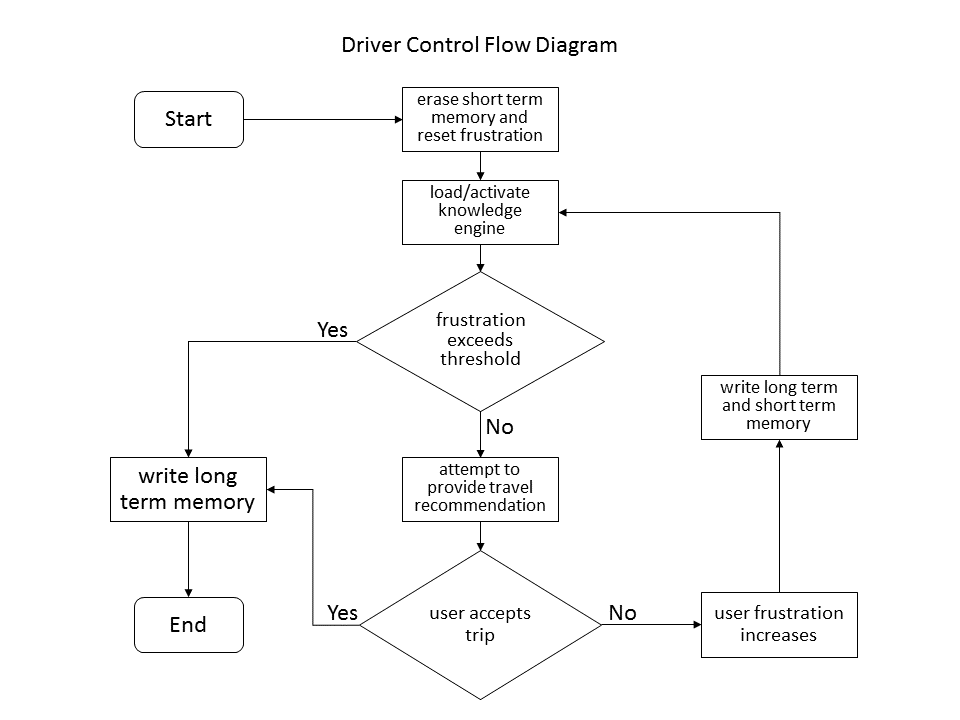
\includegraphics[width=12cm]{driver_control_flow.png}
\caption{Implemented control flow of the main driver.\label{fig:driver}}
\end{figure}

Figure \ref{fig:driver} documents the primary control of the agent. Although the details of this system will be covered within the design section, it should be noted that this process changed very little from initial discussion regarding the operation of the system. It was determined that the initial catch up phase with the user was important, and this was retained throughout development. Additionally, the early idea of programming in an exchange, whereby the agent alternates between asking questions and providing suggestions, was developed almost completely as envisioned.

Although, initially, the designs suggested needing more process diagrams, the amount of work that could be performed with the PyKE engine was underestimated. Of course, within the PyKE library, there are an extensive number of interactions occurring. However, as the PyKE library is nothing more than a tool of the system, the internal workings of PyKE will not be described here. Interested readers can explore the PyKE documentation directly\cite{pyke}.

\subsection{Influence Diagrams}
\begin{figure}[!htb]
\centering
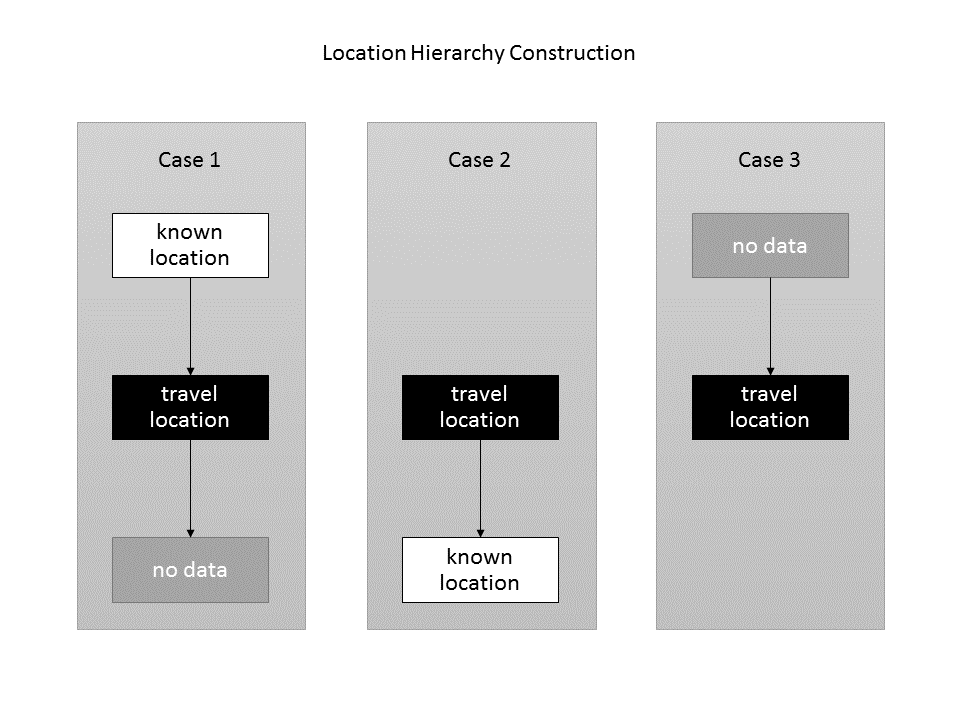
\includegraphics[width=12cm]{location_hierarchy.png}
\caption{Influence of location in the automatic building of a hierarchy.\label{fig:hierarchy1}}
\end{figure}
Influence diagrams, such as Figure \ref{fig:hierarchy1}, document the various relationships between entities in the knowledge engine. In the figure, location information is influenced by the presence of related location facts. This separates new location information into three cases.

In Case 1, the system recognizes a new travel location as a leaf node within the already existing location hierarchy. The system already knows of a larger location which encompasses the new location, and is unaware of a location specifying the location with higher granularity.

Case 2 represents a scenario where the system is aware of the travel location, but is also aware of more specific locations within this location. For example, if the user states they traveled to South American, the system would recognize this a non-specific location due to knowledge already known of locations within South America. This would cause the system to inquire where in South America the user traveled.

Case 3 represents the reverse situation from Case 2. The user has specified a location which is specific enough that the system is unaware of it. It is, essentially, a new entry. In this case, the agent prompts the user for the more general location which contains the original location, and continues prompting for more general locations until it is able to establish the location within the hierarchy. As an example, if the user specifies ``Boston'', and if the system has not recorded ``Boston'' previously, the system will ask for a more general location. The user may then specify either ``Massachusetts'', ``United States'' or some other location. ``United States'' is most likely in the knowledge engine, but ``Massachusetts'' may not be. In the later case, the system would patiently prompt for the more general location of ``Massachusetts'', at which point most users would type ``United States'', thus establishing the location of ``Boston'' in the location hierarchy. It is important to note that the system does not recognize items as specifically \emph{countries} or \emph{cities}, but rather, reasons about locations only by which locations are above or below it in the hierarchy. 

\section{Design}
\subsection{Overall Architecture}
The Travel Buddy is written in Python and is designed to be
compatible with version 2.7. Porting the code to
Python 3 could be done with little effort. The primary
library at use in the program is PyKE (Python Knowledge
Engine), for which there are version compatible with both
Python 2.6+ and Python 3. As this program is a prototype,
no extra effort has been invested in developing a
user interface. Instead, all I/O is handled through a simple
commandline interface relying on stdin and stdout.

The components of the program can be broken into several
parts, many of which are mandated by the PyKE library.

\subsubsection{Driver}
The driver (implemented in the file driver.py) handles the
basic control flow of a user interaction with the system.
The driver starts the knowledge engine and 
segments the types of interactions available
with the knowledge engine and assists in modeling the
user. Additionally, since PyKE allows forward-chaining to
occur only once for each engine, the driver handles the
creation of multiple engines based on the same knowledge
base in order to facilitate different executions of
forward-chaining rules.

As Figure \ref{fig:driver} shows, the driver begins by erasing the short term memory file and setting the user frustration level to zero. Following these initialization steps, the knowledge engine is activated for the first time. Within the knowledge engine, a number of forward chaining rules run to initialize the session and acquire knowledge about the user. After the completion of the forward chaining rules, the user frustration level is compared to the threshold and the program exits if it is determined the we have been unable to suggest a trip in a reasonable time.

Assuming frustration is within guidelines, the driver attempts to prove a number of backward chaining ``recommenders''. These rules are successfully proved when the knowledge engine finds a trip meeting the recommendation criteria \emph{and} the user indicates they would enjoy the trip. Therefore, if any of the rules can be proved, the program is complete.

If none of the recommenders are proven, the frustration level is increased. Short term memory and long term memory are both written to disk. The existing knowledge engine is deleted and a new one is created. Recreating the knowledge engine activates the forward chaining rules again, which respond by asking further questions of the user, after which the backward chaining rules again fire. Through this iterative process, the driver attempts to alternate between learning about the user, and suggesting places the user may enjoy. The frustration level guards against boring the user when the Travel Buddy is unable to be useful.

\subsubsection{Memory}
The memory of the Travel Buddy is split into two files, \texttt{shortterm.kfb} and \texttt{longterm.kfb}. Both files are implemented as PyKE Knowledge Fact Base files and, therefore, consist of names attached to tuples of values, where each name/tuple pair represents a piece of knowledge for the system.

The long term memory contains knowledge which is carried over from session to session. It contains facts about users who have previously logged into the system, such as: name, places traveled to, activities enjoyed, weather preferences, and friends. There are also facts about locations and their location within a global hierarchy. The final primary category of facts are those about activities, which specify which locations have certain activities and other minor details.

During each session the system adds appropriate details to the long term memory as facts are learned from the user. For example, if the user answers that they like surfing, the system would record into the long term memory a fact relating the user to enjoying surfing. The long term memory, therefore, contains extensive data about all users who have logged into the system.

The short term memory is used for temporary storage during each session. It contains many different kinds of facts. Certain system facts are stored in short term memory to track from where in the driver the knowledge engine is being activated. Other facts, such as those about the current user of the system and interaction with user during a session, are also stored in the short term memory. Finally, the short term memory is used for saving inferred knowledge which may take up lots of space and can easily be inferred again during later sessions.

Separating the memory into these two areas was necessary due to the nature of how PyKE operates. PyKE runs all forward chaining rules at one time, during activation, before returning control to the driver. Because our system then attempts to obtain additional knowledge from the user, any learned knowledge will not be processed by PyKE without reloading the engine. Therefore, to preserve the short term ``session knowledge'', we put these facts in to the short term knowledge fact base. This fact base can then be activated after the engine is reloaded and our learned knowledge is restored.

\subsubsection{Rules}

There is one rule base for the system, contained within a file named \texttt{travelrules.krb}. The rules are written in PyKE's knowledge rule base syntax and consist of both forward chaining and backward chaining rules.

Some rules are simple forward chaining inference rules.
For example:
\begin{Verbatim}[xleftmargin=2.5cm]
associative_property_of_friendship
    foreach
        longterm.friends($person1, $person2)
    assert
        longterm.friends($person2, $person1)
\end{Verbatim}

The rule simply assumes that friendship is two-way. If we have learned that a user is friends with someone else, this will infer the reverse relationship.

In addition to the straightforward rules, there are many more complicated rules. As mentioned previously, PyKE breaks rules into forward chaining and backward chaining.

Forward chaining rules are all run when the rule base is activated. They are run continuously until none of the preconditions hold for any forward chaining rules. These rules can also assert facts, thus adding knowledge to the engine.

Backward chaining rules are not run automatically by PyKE. Individual rules must be selected and the knowledge engine attempts to prove these rules by satisfying their arguments. During the proving process, the knowledge engine will often need to prove other backward chaining rules and look up facts from the fact bases. The knowledge engine then responds with either a proof or an error.

It is important to note that the PyKE system does not allow the backward chaining rules to assert new facts into the fact bases, nor will the forward chaining rules run after the initial rule base activation. It is possible to write facts into the fact base, however, they will not be used until the next activation of the rules.

\subsubsection{Questions}
A strong feature built-in to PyKE is its system for automatically asking questions of the user as needed. Any questions can be written into a knowledge question base. Each question has a unique name. These questions can then be used in both the forward chaining and backward chaining rules. When a rules encounters a question, it proceeds to prove it as it would any other condition. If the question variables are already bound, the question fails if the user answer does not match the bound value. If the variable is unbound, the user answer is bound to the variable and the question succeeds.

Having this feature integrated into PyKE greatly eased the process of implementing a basic user interface. It also allows a much larger portion of the processing to be performed entirely within the knowledge engine. In turn, this reduced the number of times the rules base needed to be recompiled and reloaded.

The following is the basic syntax of all questions:
\begin{Verbatim}[xleftmargin=2.5cm]
confirm_recommendation($place, $ans)
    I think you would have a really good time in $place.
    Do you think I'm right?
    ---
    $ans = yn
        True ! I thought so.
\end{Verbatim}

Arguments can be referenced within the question and the response can be bound to an argument, as well. In addition, a canned response, based on the answer provided, can be displayed to the user. The example above shows all these features used together.

\subsection{User Modeling}

As the user model was a focal component of this system, we placed significant effort into learning, representing, and remembering information about the user. In fact, beyond simply developing a model of the user during an interactive session, we remember information about all users of the system and store a great deal of information about each user into long term memory.

For each user, we retain the following information in long term memory:
\begin{multicols}{2}
\begin{itemize}
\setlength\itemsep{0em}
\item Name
\item Login dates
\item Locations traveled
\item Activities liked
\item Friends
\item Location of residence
\item Possessions related to activities
\item Languages spoken
\end{itemize}
\end{multicols}

Some aspects of the user model, such as languages spoken, have not been implemented into any of the rules. Despite this, the facts have been left in the long term memory as a way of documenting possible directions for future work. In fact, the relative ease with which facts can be stored in the system allows expansion of the system to incorporate any variety of facts pertaining to the user.

In addition the the long term storage of user data, several short term attributes are retained for the current user of the system.

The most important of the short term attributes is that of frustration. Since our system does not attempt to optimize its travel recommendations and, instead, provides a more conversational manner of proposing trips, it was necessary to determine if we were being boring or simply unhelpful to the user. We model this as frustration. The value of frustration is initialized to zero and is only ever increased, much the way guilt has been modeled in other cognitive systems\cite{arkin09}. Although this is a simplistic representation, it servers ensure that the ``buddy'' doesn't continue making suggestions when the user is unhappy with the suggestions.

The user model is used during almost every step of the systems operation. The current user is the first fact stored into short term memory. Next, the initial dialog with the user is used to insert new facts about the user. Later in the session, as the system suggests places, the user model of activity likes, previous travel locations, and weather preferences are all used in an attempt to provide a good travel suggestion. Finally, when the user does not accept a proposal, the system attempts to learn more about the user before providing another suggestion.

Although the user model is simple, it has proven adequate for the current state of the system. It would be easy to expand the user model to include other attributes, as we document in the future works section.

\subsection{Planning Logic}
Every session with a given user begins by erasing the short term memory and then activating the knowledge rule base. In doing this, the knowledge engine loads all the facts from the knowledge fact bases and begins running the forward chaining rules.

The first rule to fire always prompts for, retrieves, and stores, the name of the current user. Following this trivial step, the begins a friendly ``catch up'' dialog. During the dialog, the system asks if the user has been on a recent trip and, if so, asks for details about the trip. This step mimics a conversation with a friend who has not been seen in a while and who simply want to know what's been happening.

After the dialog ends, the system consults all the facts known about the user. A series of backward chaining ``recommender'' rules are tested. This process results in the user possibly being presented with a trip based on the user model and a certain amount of randomness. The randomness is in place to ensure that each recommender rule is only used with a certain probability, thus preventing the same rule from being used every time.

If the user accepts the proposed travel destination, the program terminates, happy to have proposed an acceptable destination. Otherwise, the system attempts to learn something new about the user before proposing another destination.

Throughout the session, if the proposed destinations are rejected by the user, the system models this by increasing the frustration value in the user model. When the frustration level exceeds a threshold level, the agent ``bows out'' of the conversation by saying that it seems to be unable to assist the user in selecting a destination.

An important aspect of our agent is that not all interactions are successful. The goal was to create an agent which was interactive and interesting, while also providing educated recommendations. However, despite sometimes receiving ``silly'' recommendations, the underlying rules are based on a solid user model. It is hoped that this form of interaction is more rewarding for the user, as if talking with a friend who occasionally says something funny.


\subsection{Operations}

In order to build a working system, we will need different operations in order to deal with both interpreting the user input, retaining the informations gained from the interpretation and the mapping and then providing some kind of response. For our system we imagine there would be two different kinds of responses, questions and suggesting. Questions have the purpose of directly asking the user in order to clarify things for the user model. Suggestions can be served up as direct suggestions or be formulated as fabricated previous experiences for the agent to which the user can respond positively or negatively, thereby also providing insight to the user's preferences.
We want to present these responses mostly at random in order to avoid making the conversation follow a set pattern.


Our simple interpretation system would work by receiving some user input. Since we are not implementing an extensive natural language processing system, the next step would be to extract known keywords from the input, such as destination names and simple adjectives. Next, we will attempt to extract coherent facts from the keywords and save them to our knowledge base. So if the user inputs "I went to Tahiti. I love Tahiti!"  we save the fact that the user went to Tahiti in our knowledge base and another fact about how they see that destination in a very positive light. If there is some difficulty extracting facts from the keywords, perhaps because of conflicts, we might try to clarify by asking the user directly by presenting what the agent deems the most appropriate interpretation and getting their response. If the user does not accept the interpretation, the agent could try presenting another interpretation or just give a confused response.

The user might also add general information about destinations or their personalities using these adjectives. By saying "I'm very adventurous.", the agent would update its facts by now adding the fact that they are adventurous. Or they could describe a destination as being relaxing or educating, which would in turn add more detail to the descriptions we have of certain trips.


All of these gathered facts are then sometimes used for making suggestions or asking questions. We could for example use the fact that they went to Tahiti and liked it there to look up destinations which share the same characteristics. For this we have a collection of facts about the different destinations. So Tahiti might have a fact categorizing it as being a tropical destination. Doing simple matching, we might just end up pulling another destination which has this fact and suggesting it. During the matching process we will also try to filter out destinations which have characteristics which are seen negatively by the user. We can either completely rule them out or perhaps base our suggestions around a scoring system based on the features, such that some destinations are allowed despite their shortcomings.


Generally the knowledge base is updated whenever the agent has an interpretation it is sure of which adds more information. Knowledge is retrieved when making suggestions or asking the user about their experiences or preferences.


\section{Practical}

\subsection{The Current System}
\begin{figure}[!htb]
	\begin{subfigure}[b]{0.48\textwidth}
		\centering
		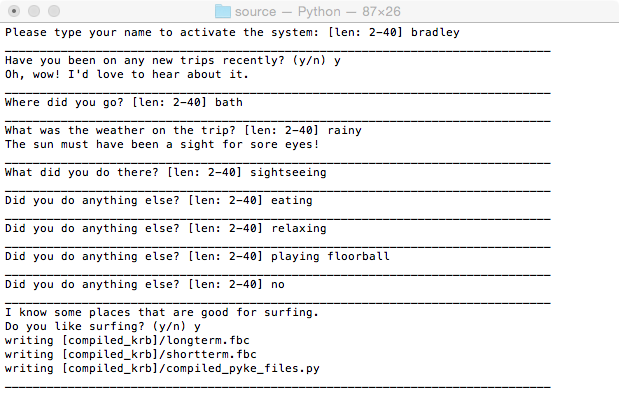
\includegraphics[width=\textwidth]{system2.png}
		\caption{ }
	\end{subfigure}
	\hfill	
	\begin{subfigure}[b]{0.48\textwidth}
		\centering
		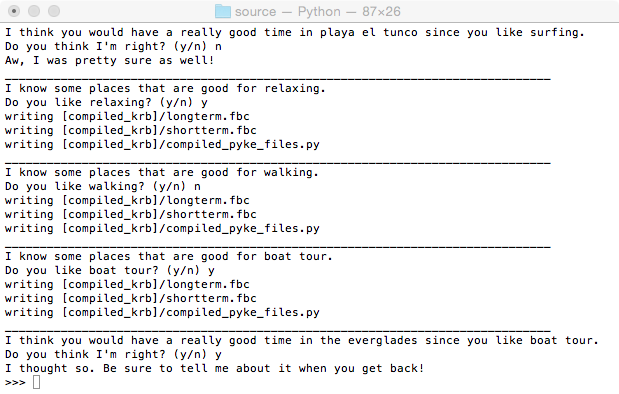
\includegraphics[width=\textwidth]{system1.png}
		\caption{ }
	\end{subfigure}
	\caption{Screenshots of the running system.}\label{fig:system}
\end{figure}
Figure~\ref{fig:system} shows an example of the running system after all forward chaining rules have been run. The system will first prompt for a user name and ask about any recent trips the user has been on. All information that is provided in this section will later be saved into longterm memory and will be available for future runs of the system. This means that every use of the system will extend the database of travelfacts.
After acquiring these initial facts about the user, the system will then proceed to recommend locations to the user with a reason why this location was selected, or ask about their opinion on certain randomly selected activities. If a recommendation was not accepted it will not recommend anything new before it has gathered more information about the user.

\subsubsection{Strength and Weaknesses}
The system shows very good results with respect to matching activities of a location to activities that the user liked, or activities of places the user has visited before. This means the selected recommendations are always relevant to the user's interest and never completely random.
The integration of the weather conditions of a particular location into the recommendation process is still lacking which we mostly attribute to the lack of information about the weather in the database which can easily be fixed by adding those facts to longterm memory.
Recommendations can feel a bit random at times since the system considers all the information it has collected about the user when choosing a location and doesn't place more relevance on more recently acquired data.
Once it has recommended a location and said location was rejected it will not recommend it again. So it will not pester the user to go to a specific location over and over again.
Apart from the recommendation part of the system, the goal of providing a conversation like experience was not entirely reached. This is mostly due to PyKE's question/answer style of acquiring knowledge which does not lend itself easily to realize a natural feeling conversation. The questionbase does provide a good starting point though and could later be replaced by a natural language interface.

\subsection{Future Work}
The system has a lot of potential in various areas. 
Obviously the recommendation based on the weather condition needs improvement which could likely be achieved by extending the factbase by providing weather information about the various locations in longterm memory.
Naturally an extension of the factbase with respect to locations and location characteristics will provide more variety in the recommendations.
Another obvious and easy extension might be to have the system display all the information about the current user that is already in the database after they entered their name to provided an overview of what the system already knows about the user. 
Adding more characteristics to the user model, like relationships (friends, etc.), their inventory, or maybe the languages they speak, and use these facts for the matching process in a similar manner as for liked activities would make the recommendation process more interesting.
In a similar way, similarities between places could be inferred by weather conditions, features, spoken language or geographical location.
The way we contain locations in our system allows for quick learning of hierarchies. However, since we lack information about locations, such as whether they are a city, country or continent, the agent lacks a degree of nuance in that area.
While recommending the most specific place to the user works fine, being able to also recommend countries or cities in some cases would make the agent more believable. When people talk about traveling, 
often times they don't talk about specific cities on their own, they talk about the area or country. With our current system of simple hierarchical relations, we could still generate sentences such as "Denver, Colorado". 
But by keeping track of the category of a location, we could generate sentences such as "The city of Denver is in the state of Colorado." and we would be able to change up our recommendation to sometimes suggest locations 
with a lower specificity. A concrete case where this could be applied would be if a location is not well traveled. If the agent finds that few users have traveled to the location it is recommending, it could sometimes instead 
reduce the level of specificity to recommend something more general. Or it could use the information gathered about the location to also present it in relation to another area which contains it. This would make 
a recommendation feel more natural and engaging, as the agent would do what most people do if they are talking about obscure topics. In order to implement this, the agent would only need to ask what kind of location it is when a new location is presented by the user.
We did not implement this because we thought of it much later in the process of the implementation, making it too late to revamp the system. Since it was not vital, we did not put much focus into this.
We could also determine the size of a location (i.e. if it is a city, a region or a country) from its place in the location hierarchy, and recognize places that were spelled differently but obviously mean the same thing such as 'the united states of america' and 'the usa'.


During the development of our system, we experimented with different approaches in order to make the agent as engaging as possible. To make the interaction feel more like a conversation than the current question/answer game we will integrate NLTK, python's natural language toolkit, to provide a user interface with the capability to process natural language and infer travelfacts and user likes and dislikes from the conversation. 
During development a simple interpreter was built in python, using the NLTK package wordnet. 
The interpreter component would have a small vocabulary based on words often used when talking about travel. Interpretation would be done word by word, matching each word to 
the vocabulary or to a set of synonyms generated by wordnet. A match would associate annotations with the word and would improve the overall score of a sentence in regards to said annotations.
Lastly it would attempt to use the knowledge base in order to match words which fell through the initial vocabulary and synonym check, in order to match proper nouns and activities. 
The result was then a set of annotations, which could be matched against one of the predefined cases, such as expressing a preference, talking about having traveled somewhere or describing oneself. 
These cases would then contain an action the agent could perform in order to react to the given input. The reason why we did not integrate this into the final version was because the agent mostly takes charge on its own, while the component was 
written with the opposite in mind. There is also the fact that it was difficult integrating the pure python interpreter into the PyKE rules and questions, as PyKE mostly handles the user input through 
the questions it presents the user. The question file allows almost no tinkering, outside of presenting exact match answers or answers for patterns.

Natural language processing would also allow the user to ask questions themselves and inquire about the overall location of a recommended place, for example the country or region it is in. Or the user could ask for specific activities of a place they are interested in, or other activities you can do at the recommended location. In relation to our recommenders, we also attempted to add some variety by optimizing the place suggested to the user, such that the agent could sometimes suggest a location which had the highest 
number of activities the user might enjoy instead of just one. At a simpler iteration of the system we got it to work, but it stopped producing results later after ensuring that the agent does not 
recommend something it has already recommended in the same session. This may be due to the many new constraints imposed on a candidate location. Suggesting the very best match relied on 
finding a location such that no other location would have a higher score of activities. This also means that the secondary locations need to be constrained such that we can still find results 
if the user has already been to the very best location or we have already recommended such a place. Otherwise, the agent would conclude there is no better match and do nothing. While this was 
accounted for, the issues still persisted and the method was abandoned. This may also be because of the specificity constraint on locations. Without the constraint, any match would lose to locations such as 'earth',
 since such locations contain a high number of activities.

 
\subsection{The Team}
\subsubsection{Paul}
% main part of  the coding work
% provided travelfacts longterm 
% report: design component
\subsubsection{Diana}
% nltk module that we lacked time to integrate into the main code
% improved recommendation process
% report: design, operations (4.4)
\subsubsection{Inga}
Apart from the initial proposition and discussions about the systems capabilities, requirements and design, Inga provided the longterm memory with a multitude of travelfacts that were extracted from the travelblogs that were mentioned in the report. 
Additionally to that, she wrote extensions to the travelquestions and travelrules. 
For the report she wrote the Practical section, reworked the Introduction section, added citations and fixed spelling and grammar mistakes throughout the whole file.
% provided travelfacts longterm 
% extensions of code (questions and rules)
% report: practical, improve motivation, added citations to related work

\begin{thebibliography}{9}

\bibitem{amanda15}
Amanda (2015) \emph{A dangerous business travel blog}. www.dangerous-business.com
\bibitem{arkin09}
Arkin, A. C., \& Ulam, P. (2009). \emph{An ethical adaptor: behavioral modification derived from moral emotions}. Proceedings of the Eighth IEEE International Conference on Computational Intelligence in Robotics and Automation (pp. 381-387). IEEE Press.
\bibitem{cavazza08}
Marc Cavazza, Cameron Smith, Daniel Charlton, Li Zhang, Markku Turunen, and Jaakko Hakulinen. 2008. \emph{A `companion' ECA with planning and activity modelling}. In Proceedings of the 7th international joint conference on Autonomous agents and multiagent systems - Volume 3(AAMAS '08), Vol. 3. International Foundation for Autonomous Agents and Multiagent Systems, Richland, SC, 1281-1284.
\bibitem{kate15}
McCully, Kate. (2015) \emph{Adventurous Kate's solo female travel blog}. www.adventurouskate.com
\bibitem{loper02}
Loper, Edward, and Steven Bird. \emph{NLTK: The natural language toolkit}. Proceedings of the ACL-02 Workshop on Effective tools and methodologies for teaching natural language processing and computational linguistics-Volume 1. Association for Computational Linguistics, 2002.
\bibitem{pyke}
Frederiksen, Bruce. (2009). \emph{PyKE python knowledge engine}. pyke.sourceforge.net
\bibitem{ricci02}
Ricci, Francesco, et al. \emph{ITR: a case-based travel advisory system}. Advances in Case-Based Reasoning. Springer Berlin Heidelberg, 2002. 613-627.


\end{thebibliography}

\end{document}
